%------------------------------------------------------------------------------
% Template file for the submission of papers to IUCr journals in LaTeX2e
% using the iucr document class
% Copyright 1999-2013 International Union of Crystallography
% Version 1.6 (28 March 2013)
%------------------------------------------------------------------------------

\documentclass[preprint]{iucr}              % DO NOT DELETE THIS LINE

     %-------------------------------------------------------------------------
     % Information about journal to which submitted
     %-------------------------------------------------------------------------
     \journalcode{J}              % Indicate the journal to which submitted
                                  %   A - Acta Crystallographica Section A
                                  %   B - Acta Crystallographica Section B
                                  %   C - Acta Crystallographica Section C
                                  %   D - Acta Crystallographica Section D
                                  %   E - Acta Crystallographica Section E
                                  %   F - Acta Crystallographica Section F
                                  %   J - Journal of Applied Crystallography
                                  %   M - IUCrJ
                                  %   S - Journal of Synchrotron Radiation
\usepackage{graphicx}
\usepackage[T1]{fontenc}
\usepackage[utf8]{inputenc}
\usepackage{amsmath}

\begin{document}                  % DO NOT DELETE THIS LINE

     %-------------------------------------------------------------------------
     % The introductory (header) part of the paper
     %-------------------------------------------------------------------------

     % The title of the paper. Use \shorttitle to indicate an abbreviated title
     % for use in running heads (you will need to uncomment it).

\title{Application of signal separation to diffraction image compression and serial crystallography}
%\shorttitle{Short Title}

     % Authors' names and addresses. Use \cauthor for the main (contact) author.
     % Use \author for all other authors. Use \aff for authors' affiliations.
     % Use lower-case letters in square brackets to link authors to their
     % affiliations; if there is only one affiliation address, remove the [a].

\cauthor[a]{Jérôme}{Kieffer}{jerome.kieffer@esrf.fr}{}
\author[a]{Julien}{Orlans}
\author[a]{Nicolas}{Coquelle}
\author[a]{Samuel}{Debionne}
\author[b]{Shibom}{Basu}
\author[a]{Alejandro}{Homs}
\author[a]{Gianluca}{Santoni}
\author[a]{Daniele}{De Sanctis}

\aff[a]{European Synchrotron Radiation Facility;71, avenue des Martyrs;CS 40220;38043 Grenoble Cedex 9 \country{France}}
\aff[b]{EMBL Grenoble; 71 avenue des Martyrs; CS 90181; 38042 Grenoble Cedex 9; \country{France}}

     % Use \shortauthor to indicate an abbreviated author list for use in
     % running heads (you will need to uncomment it).

%\shortauthor{Soape, Author and Doe}

     % Use \vita if required to give biographical details (for authors of
     % invited review papers only). Uncomment it.

%\vita{Author's biography}

     % Keywords (required for Journal of Synchrotron Radiation only)
     % Use the \keyword macro for each word or phrase, e.g. 
     % \keyword{X-ray diffraction}\keyword{muscle}

\keyword{background extraction}
\keyword{serial crystallography}
\keyword{peak-picking}
\keyword{lossy compression}

     % PDB and NDB reference codes for structures referenced in the article and
     % deposited with the Protein Data Bank and Nucleic Acids Database (Acta
     % Crystallographica Section D). Repeat for each separate structure e.g
     % \PDBref[dethiobiotin synthetase]{1byi} \NDBref[d(G$_4$CGC$_4$)]{ad0002}

%\PDBref[optional name]{refcode}
%\NDBref[optional name]{refcode}

\maketitle                        % DO NOT DELETE THIS LINE

\begin{synopsis}
Precise background assessment and application to single crystal image compression and serial crystallography data pre-processing. 
\end{synopsis}

\begin{abstract}

We present here a real-time analysis of diffraction images acquired at high frame-rate (925 Hz) and its application to macromolecular serial crystallography.
The software uses a new signal separation algorithm, able to distinguish the amorphous (or powder diffraction) component from the diffraction signal originating from single crystals. 
It relies on the ability to work efficiently in azimuthal space and derives from the work performed on pyFAI, the fast azimuthal integration library.
Two applications are built upon this separation algorithm: a lossy compression algorithm and a peak-picking algorithm; the performances of both is assessed by comparing data quality after reduction with XDS and CrystFEL.


\end{abstract}


     %-------------------------------------------------------------------------
     % The main body of the paper
     %-------------------------------------------------------------------------
     % Now enter the text of the document in multiple \section's, \subsection's
     % and \subsubsection's as required.

\section{Introduction}

X-ray macromolecular crystallography is one of the most successful methods to determine the atomic structure of biological molecules. 
The achievable diffraction quality may often be limited by radiation damage. 
Although cryogenic conditions permit to extend the lifetime of crystals in the X-ray beam and to increase the maximum absorbed dose before inducing damage they may hinder physiologically relevant conformations. 
This limitation has renovated the interest for room temperature macromolecular crystallography by applying a more drastic approach to overcome the radiation damage problem by collecting data from thousands of small crystals, in what became known as serial crystallography. 
First developed at X-ray free electron laser sources (\textsc{xfel}) \cite{Chapman2011, structure_sx} the method is currently applied also at synchrotron sources \cite{ssx, ssx_desy, ssx_id13, ssx_diamond}.


% The diffraction quality achievable from a macromolecular crystallography experiment is limited by radiation damage.
% %we can cite here Garman and Weik
% To achieve a complete dataset from a single crystal, data collection happens in a cryo-cooled environment. 
% Exposure time has in any case to be limited due to radiation damage. 
% This issue is even stronger at room temperature.
% In room temperature macro-molecular crystallography (MX), several crystals are often needed to collect a complete dataset without compromising the resolution of the electron density map.
% A more recent approach to solve the radiation damage problem for smaller crystals is serial crystallography.
% First developed at X-ray free electron laser sources (\textsc{xfel}) \cite{Chapman2011, structure_sx} the method is currently applied also at synchrotron sources  \cite{ssx, ssx_desy, ssx_id13, ssx_diamond}.
%Crystals are exposed in a serial way to the beam with random orientation, giving making the data-reduction of

\subsection{Serial crystallography using synchrotron sources (SSX)}
%not sure we need subsections here
%Serial crystallography is a relatively new technique in structural biology. 
%It is composed of several techniques where multiple crystals (hundreds or thousands) are exposed in a serial %way to the X-ray beam to collect a complete dataset. 
%
%The serial approach is particularly useful to try to overcome the limitations of radiation damage in %rotational crystallography, particularly in very small crystals.
Serial crystallography consists in exposing thousands of small crystals to the X-ray beam only once in a serial way.
Diffraction is collected with a very high flux density, in order to extract the most information from a single shot.
This is in contrast with traditional rotational crystallography, where a complete dataset is collected from a single crystal rotated around one (or several) axis. 
Those SSX images represent a slice through the reciprocal space, thus intersect a lower fraction of the reciprocal space as the crystal is still, in comparison with rotational crystallography.
To achieve a complete dataset, thousands of frames have to be collected, individually indexed and then merged.
The high flux needed to collect all diffraction signal from a single crystal within a single exposure makes the SSX technique a good candidate to benefit from the 4\textsuperscript{th} generation synchrotron sources, such as the new ESRF-EBS update \cite{EBS}.
However, macromolecular crystallography beam-lines (MX) have been extremely specialized towards rotational data-collection and thus require modifications to the experimental setup to perfom SSX experiments.
The synchrotron serial crystallography beamline (ID29 at the ESRF) has been built to have a dedicated environment to perform SSX experiments with a high flux (using a larger energy bandwidth with a multilayer monochromator), a high-speed chopper (to separate X-ray pulses), several sample delivery methods and a fast detector.

\subsection{\textsc{Jungfrau} 4M detector}
Macro-molecular crystallography has enormously progressed in the last decades with to the introduction of photon-counting detectors \cite{pilatus}. 
With their absence of read-out noise and their fast speed, the main limitation of photon-counting detectors is the achievable count-rate, i.e. how fast the electronic of a pixel is able to count arriving photons.
% difference bewteen pixel counting vs integrating, in speed ...
Unlike photon-counting detectors such as the Eiger detector \cite{Eiger}, the \textsc{Jungfrau} detector \cite{jungfrau2016} is an integrating detector, thus, it is not limited by the count rate, even under the very intense flux expected when recording Bragg-peaks.
To cope with this photons density, every single pixel implements an automatic gain switching mechanism (3 levels) which offers a precision of the order of one third of a keV on the higher gain mode, a precision of the order of one photon in the intermediate level and the ability to cope with thousands of photons in the lower gain mode.
Moreover, the \textsc{Jungfrau} is able to operate at two kilohertz, which means the image must be read every half millisecond.
Since the \textsc{Jungfrau} detector is an integrating detector, dark current and flat-field correction have to be applied: every pixel has three, so called, pedestals and three gain values (one for each gain level). 
This large number of parameters per pixel makes the pre-processing of raw signal challenging at full speed: the signal from a single pixel, initially packed with 16 bits per pixel, gets expanded to 32 bits (floating point or integer value), doubling the required bandwidth and the storage size \cite{jungfrau_PSI}.
The ID29 beamline features a \textsc{Jungfrau} 4M detector, operating at 1kHz, pace imposed by the chopper and synchronized with the photon bunches from the ESRF.
At nominal speed, the detector will produce 16 GBytes of pre-processed data per second, making the data analysis and storage extremely challenging.

\subsection{Requirements for online data processing}

Serial crystallography is one of the techniques where online data processing is likely to have most impact:
millions of images are to be collected, and existing detector already saturate the fastest storage systems, not even considering the cost this storage.
Beside this, only a few percentage of the frames are expected to contain diffraction signal and out of them, a fraction will be indexed, integrated and thus useful to solve the protein structure.
Efficient processing of raw images is thus essential for SSX, with 4 levels of increasing complexity:
\begin{itemize}
    \item image reconstruction with pedestal correction
    \item \textit{veto-}algorithm: be able to sieve-out images with poor signal
    \item save only pixels with diffraction signal
    \item precise location of peak position with indexation \cite{toro}
    \item real-time integration of diffraction peaks
\end{itemize}.

Reconstruction and pedestal correction have been already described in \citeasnoun{lima2}.
This document will focus on the subsequent steps: the detection of signal is addressed in section 2, sparse data compression in section 3, and their application to serial crystallography in section 4 before concluding in section 5.
%The second step is to collect only pixel values corresponding to diffraction signal.
%or even an algorithm able to point.

% 1e6 images, 100k hits, 10k indexed and integrated images
% for each of the individual frame low partiallity need 10k frames/crystall to get a complete dataset with enough redundancy




\section{Algorithm for the separation of the amorphous background from the Bragg peaks}
\subsection{Background scattering}
%be careful & be precise ...
The simplest implementation of Bragg peaks separation is to assume that the background signal originates from scattering of amorphous material 
%(or from an isotropic powder), 
giving an isotropic signal that ideally presents only smooth variations.
Before background subtraction, the raw signal has to be corrected for dark noise and for any systematic anisotropic effects such as polarization corrections.
Unlike X-FEL, synchrotron X-ray beam is better characterized in energy and shows little to none pulse to pulse variability.
All anisotropic correction can be easily modelled and taken into account.
The same method can be extended to separate Bragg peaks from powder diffraction if the powder signal is isotopic, i.e. without preferred orientation. 

%the first thing is to get it working, the second is to make it fast ... coming from another field of science.
The initial implementation of signal separation in pyFAI \cite{pdj2013} was relying on a 2D polar transform followed by a median filter in the azimuthal dimension to calculate the amorphous scattering curve.
Although this method has been successfully used for large dataset analysis \cite{brocades}, it presents four major drawbacks:
\begin{itemize}
\item The 2D averaging mixes the signal originating from several pixels and blurs the signal. 
\item Pixel-splitting is needed to leverage the Moiré effect in the 2D averaging, but this further increases the blurring \cite{moire}. 
\item The 1D curve obtained after the application of the median filter shows sharp jumps from one azimuthal bin to its neighbour.
\item The median filter is computationally heavy since it is required to sort out every azimuthal bin.
\end{itemize}

We improved on this by developing a new, efficient way of performing the azimuthal averaging (including the associated uncertainty propagation). 

\subsection{Efficient azimuthal averaging and uncertainties evaluation}

\subsubsection{Pre-processing:}
The first step of the analysis consists in applying a pixel-wise correction for dark current and several normalization corrections \cite{pyfai_2020}:
\begin{equation}
\label{norm}
I_{cor} = \frac{signal}{norm}  = \frac{I_{raw} - I_{dark}}{F \cdot
\Omega \cdot P \cdot A \cdot I_0} 
\end{equation}
In  equation \ref{norm}, the numerator (referred as \textit{signal} hereafter) is the subtraction of the dark current $I_{dark}$ from the the detector's raw signal $I_{raw}$.
The denominator (hereafter \textit{norm}) is a normalization factor composed of the product of  $F$:  a factor accounting for the flat-field correction, $\Omega$: the solid angle subtended by a given pixel, $P$: the polarisation correction term and $A$: the detector's apparent efficiency due to the incidence angle of the photon on the detector plane. 
For integrating detectors, photons with high energy see longer sensor path with larger incidence angles compared to the normal thickness, thus they have a higher detection probability.
Intensity is also normalized by the incoming flux $I_0$, but being it independent from the pixel position, this correction can be applied when convenient.

\subsubsection{Azimuthal averaging:} 

Historically, the azimuthal averaging was implemented using histograms \cite{fit2d1996}.
Since the geometry of the experimental setup is fixed during the acquisition, a look-up table listing all pixels contributing to each  azimuthal-bin can be built and used to speed-up calculations \cite{pyFAI_gpu}.
The azimuthal transformation being a linear transformation, it can be implemented as a matrix multiplication, with a sparse-matrix representing the transformation and a dense vector containing the flattened view of the diffraction image. 
The compressed sparse row (CSR) matrix representation is preferred for its efficiency in performing dot products with dense vectors \cite{SpMV}.
The coefficients $c_{i,r}$ of the matrix are the fraction of area of a pixel $i$ falling into the radial bin $r$.
In the case where pixel splitting is deactivated these coefficients  ($c_{i,r}$) are always one (and zero elsewhere) since each pixel contributes to a single bin.
The sparse matrix multiplication can be used to sum efficiently values for all pixels belonging to the same bin.
The summed signal divided by the summed normalization provides the weight-averaged intensity over all pixels falling in the bin at the distance $r$ from the center, as formalized in equation \ref{avg}: 
\begin{equation}
\label{avg}
<I>_{r} = \frac{\sum\limits_{i \in bin_r} c_{i,r} \cdot signal_i}
                        {\sum\limits_{i \in bin_r} c_{i,r} \cdot norm_i} 
\end{equation}  

\subsubsection{Uncertainty evaluation from Poisson distribution.}
Photon counting detectors, such as Eiger detectors, suffer from hardly any error beside the counting uncertainty which is often referred to as Poisson statistics.
This statistical law is described by a single parameter $\lambda$ which is related to the mean $\mu$ and standard deviation $\sigma$ from a normal distribution by: $\lambda=\mu=\sigma^2$.
Other sources of noise, like the dark current noise in the case of an integrating detector,  superimpose quadratically on the Poisson noise for integrating detectors, as presented in equation \ref{poisson}:     
\begin{equation}
\label{poisson}
var_I = (\sigma_I)^{2} = <I_{raw}> + (\sigma_{dark})^{2}  
\end{equation}

During the azimuthal integration, the coefficient of the sparse matrix needs to be squared at the numerator when propagating the variance (equation \ref{varianceP}) to have uncertainties $\sigma$ proportional to the fraction of the pixel considered.
\begin{equation}
\label{varianceP}
(\sigma_{r}(I))^2 = \frac{\sum\limits_{i \in bin_r} c_{i,r}^2 \cdot \sigma_i^2}
                  {\sum\limits_{i \in bin_r} c_{i,r} \cdot norm_i} 
\end{equation}
One should distinguish the \textit{uncertainty of the mean} (sometimes referred to as the standard error of the mean, $sem$), 
which describes the precision with which the mean is known (and described in \citeasnoun{pyfai_2020}),
from the \textit{uncertainty of the pixel value} (often referred to as standard deviation, $std$) which describes the uncertainty with which the pixel value is known. 
Those two value differ only by the square root of the number of measurements in the case of an arithmetic mean: $sem = std/\sqrt{N}$ with $N$ being the number of pixel contributing to the bin.
When considering the weighted average, the previous formula becomes:
\begin{equation}
\label{sem}
sem_r = std_r \frac{\sqrt{\sum\limits_{i \in bin_r} c_{i,r}^2 \cdot norm_i^2}}{\sum\limits_{i \in bin_r} c_{i,r} \cdot norm_i}
\end{equation}
Thus, the more data points are collected, the more precisely the mean value is known but the uncertainty for a given point remains the same.
Since this document focuses on the uncertainties of pixel values, the \textit{standard deviation} will systematically be used from here on.  

\subsubsection{Uncertainty evaluation from the variance in a bin.}

Unlike photon counting detectors, most detectors do not follow the Poisson distribution and therefore the definition of a relation $\sigma^2 = f(I)$ is not simple, if possible at all. 
The integrating \textsc{Jungfrau} detector has a complex gain switching mechanism \cite{jungfrau_PSI} which makes this equation complicated.
A generic approach is proposed to measure the variance in every single azimuthal bin:

When considering the diffraction of an isotropic compound (liquid, amorphous or perfect powder), all pixels contributing to the same radial bin should see the same flux of photons (after correction of anisotropy like polarization) and the deviation to their intensities can be used to estimate the uncertainty. 
This approach is of course limited when considering the signal coming from few large crystalites (where rings becomes spotty) but it provides an upper bound for the uncertainty.
Variances (thus standard deviations) are usually obtained in a two steps procedure: one pass to calculate the average value (equation \ref{avg}) and a second to calculate the deviation to the average (equation \ref{varA}). 
This double pass approach can be implemented using sparse matrix multiplication. 
It requires twice the access to each pixel value, and extra storage space, but it is numerically robust (i.e. not prone to numerical-error accumulation).
\begin{equation}
\label{varA}
    (\sigma_{r}(I))^2 = \frac {\sum\limits_{i \in bin_r} c_{i,r}^2 \cdot norm_i^2 \cdot (\frac{signal_i}{norm_i}-<I>_r)^2}
                              {\sum\limits_{i \in bin_r} c_{i,r}^2 \cdot norm_i^2}
\end{equation}
and:
\begin{equation}
\label{varB}
(\sigma_{r}(<I>))^2 = \frac{\sum\limits_{i \in bin_r} c_{i,r}^2 \cdot norm_i^2 \cdot (\frac{signal_i}{norm_i}-<I>_r)^2}
                         {(\sum\limits_{i \in bin_r} c_{i,r} \cdot norm_i)^2}  
\end{equation}


Single pass implementations of variance calculation are faster than double pass ones since they access pixels only once and offer, in addition, the ability to perform parallel reductions \cite{Blelloch}, i.e. work with blocks of pixels.
\citeasnoun{variance2018} present a complete review on the topic, which introduces a formalism adapted here for crystallography.
Assume the weight for a pixel being $\omega_i = c_i \cdot norm_i$.
If $P$ is a partition of the ensemble of pixels falling into a given azimuthal bin, let $\Omega_{P}$, $V_{P}$ and $VV_{P}$  
be the sum of weights (Eq \ref{omega}), the weighted sum of $V$ (Eq. \ref{Vp}) and the weighted sum of deviation squared (Eq \ref{VVp}) over the partition $P$: 
\begin{equation}
\label{omega}
\Omega_{P} = \sum\limits_{i \in P} \omega_i = \sum\limits_{i \in P} c_i \cdot norm_i 
\end{equation}
\begin{equation}
\label{omegaomega}
\Omega\Omega_{P} = \sum\limits_{i \in P} \omega_i^2 = \sum\limits_{i \in P} c_i^2 \cdot norm_i^2 
\end{equation}
\begin{equation}
\label{Vp}
V_{P} = \sum\limits_{i \in P} \omega_i \cdot v_i =  \sum\limits_{i \in P} c_i \cdot signal_i
\end{equation}
\begin{equation}
\label{VVp}
VV_{p} = \sum\limits_{i \in P} \omega_i^2 \cdot (v_i - V_{P}/\Omega_{P})^2 
\end{equation}

The weighted average and associated variances are then expressed as:
\begin{equation}
\label{weighted_avg}
<I>_P = \frac{V_{P}}{\Omega_{P}} =  \frac{\sum\limits_{i \in P} c_i \cdot signal_i}
                        {\sum\limits_{i \in P} c_i \cdot norm_i} 
\end{equation}
\begin{equation}
\label{std2}
std^2 = (\sigma_P(I))^2 = \frac{VV_{P}}{\Omega\Omega_{P}}
\end{equation}
\begin{equation}
\label{sem2}
sem^2 = (\sigma_P(<I>))^2 = \frac{VV_{P}}{\Omega_{P}^2}
\end{equation}

In this formalism, equations \ref{avg} and \ref{weighted_avg} on one side and equations \ref{varA} and \ref{std2} are actually equivalent.
\citeasnoun{variance2018} present the way to perform the union of two sub-partitions $A$ and $B$ of a larger ensemble which opens the doors to parallel reductions, which are especially efficient when implemented on GPU:
\begin{equation}
\label{union_omega}
\Omega_{A \cup B} =  \Omega_{A} + \Omega_{B} 
\end{equation}
\begin{equation}
\label{union_valeur}
V_{A \cup B} =  V_{A} + V_{B} 
\end{equation}
\begin{equation}
\label{union_variance1}
VV_{A \cup b} =  VV_{A}  +  \omega_b^2(v_b-\frac{V_A}{\Omega_A})(v_b-\frac{V_{A\cup b}}{\Omega_{A\cup b}})
\end{equation}
\begin{equation}
\label{union_variance2}
VV_{A \cup B} \approx  VV_{A} + VV_{B} +  \frac{\Omega\Omega_{B}(V_A\cdot \Omega_B-V_B\cdot \Omega_A)^2}{(\Omega_{A\cup B}.\Omega_A.\Omega_B^2)}
\end{equation}
%\frac{(\Omega_{A} \cdot V_{B} - \Omega_{B}\cdot V_{A})^2}{V_{A \cup B} \cdot  V_{A} \cdot V_{B}}
While equations \ref{union_omega} and \ref{union_valeur} are trivial, equation \ref{union_variance1} describes the nominator of the variance of an ensemble when adding an extra member $b$ to the $A$.
Unfortunately, the slight difference of formalism between \citeasnoun{variance2018} and this work prevent some simplification to occur and leads to the approximate numerator of the variance ($VV$) in the case of the union of two ensemble $A$ and $B$ (eq. \ref{union_variance2}, used in OpenCL reduction \footnote{see https://github.com/silx-kit/pyFAI/blob/main/doc/source/usage/tutorial/Variance/uncertainties.ipynb}.
A numerical stability issue can arise from it when $V_A$ or $V_B$ are very small and this issue is addressed by using double-precision arithmetic when implemented on CPU and double-word arithmetic when running on GPU \cite{double_word}.

\subsubsection{Comparison of uncertainty models:}
Figure \ref{fig_std} (right hand side) presents the uncertainties (for the pixel value) as calculated from a background frame with pure Poisson noise (displayed on the left hand-side, synthetic data) using the two algorithms previously described: the Poisson model or calculated from the variance in the azimuthal bin.
% either the Poisson model or extracted from the variance in the azimuthal bin. 
While the two curves show similar amplitude, except in the corner of the detector where very few pixels contribute to each of the azimuthal bin, the variability of the ``azimuthal'' model is much more important from one bin to the neighboring one.
\begin{figure}
\label{fig_std}
\begin{center}
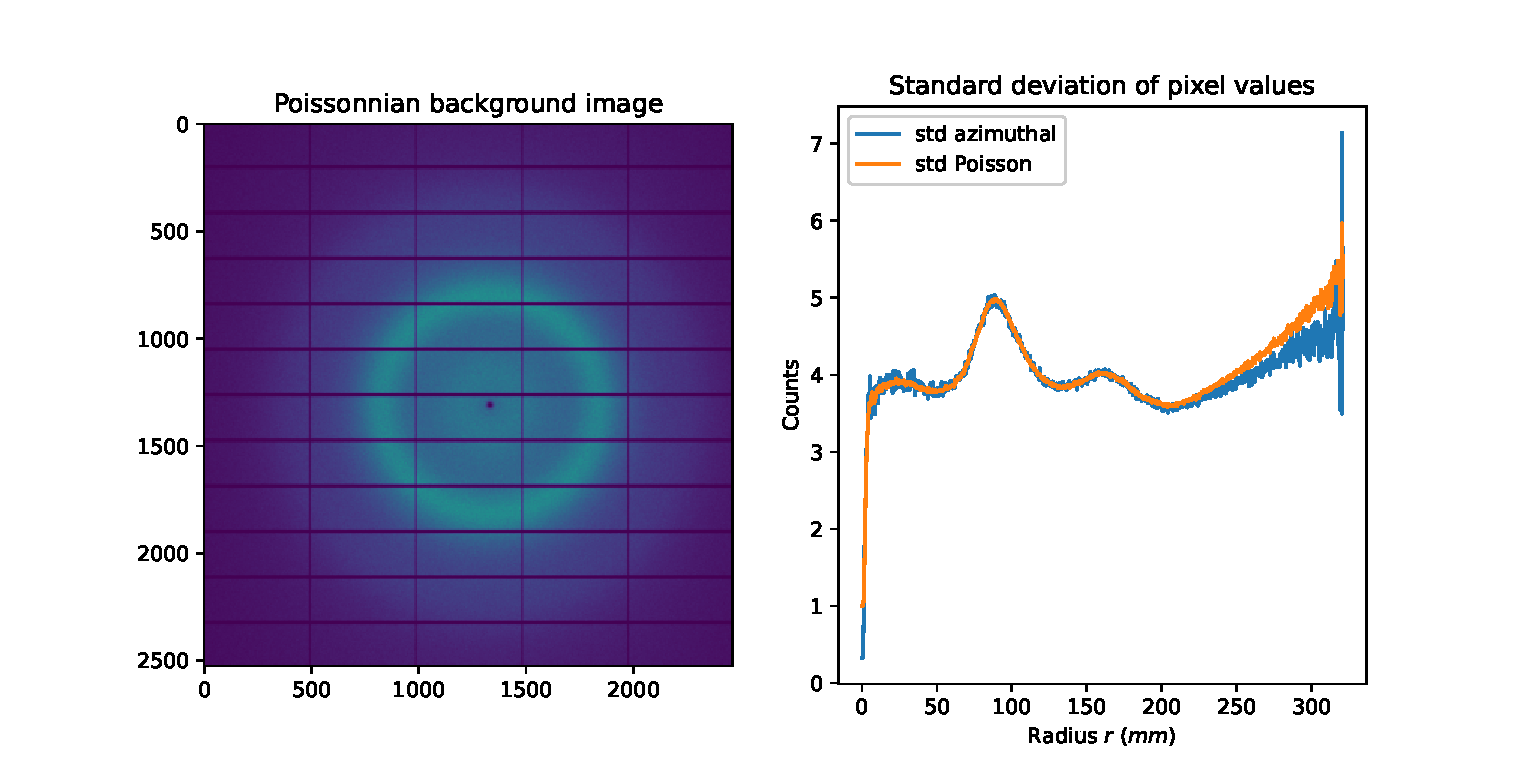
\includegraphics[width=14cm]{fig_std}
\caption{(a) Simulated diffraction frame with pure azimuthal Poisson noise of a Pilatus 6M detector and (b) uncertainties for pixel intensity as measured with the distance to the mean (azimuthal-model, blue) or from the Poisson model (orange).}
\end{center}
\end{figure}

\subsection{Histogram intensity }

The figure \ref{fig1} presents the diffraction from a single crystal of insulin collected with a Pilatus 6M detector (Fig \ref{fig1}a) and several curves obtained from azimuthal integration of those data: 
figure \ref{fig1}b is the azimuthally integrated signal (blue curve) where Bragg peaks are seen as spikes on top of a smooth background.
figure \ref{fig1}c presents the uncertainties measured according to the Poisson distribution (orange curve) %, valid since Pilatus are photon counting detectors) 
or the deviation in the ring (blue curve). 
The later presents much larger values since Bragg peaks contribute a lot to the deviation despite they represent few pixels: this highlights the sensitivity of the mean/std to outliers.
In the figure \ref{fig1}d are presented histograms of pixel intensity for pixels laying at 87mm and 160mm from the beam center. 
Each of those histograms is composed of a bell-shaped distribution with 
%negative outliers tagged with the pixel value -1 (this is specific to the Pilatus detector), and 
few positive outliers which are usually Bragg peaks.   
Those histograms in figure \ref{fig1}d have been fitted with a Gaussian curve and both the center ($\mu$) and the width ($\sigma$) of the curve match 
roughly with the average (in \ref{fig1}b) and uncertainties (in \ref{fig1}c).  
\begin{figure}
\label{fig1}
\begin{center}
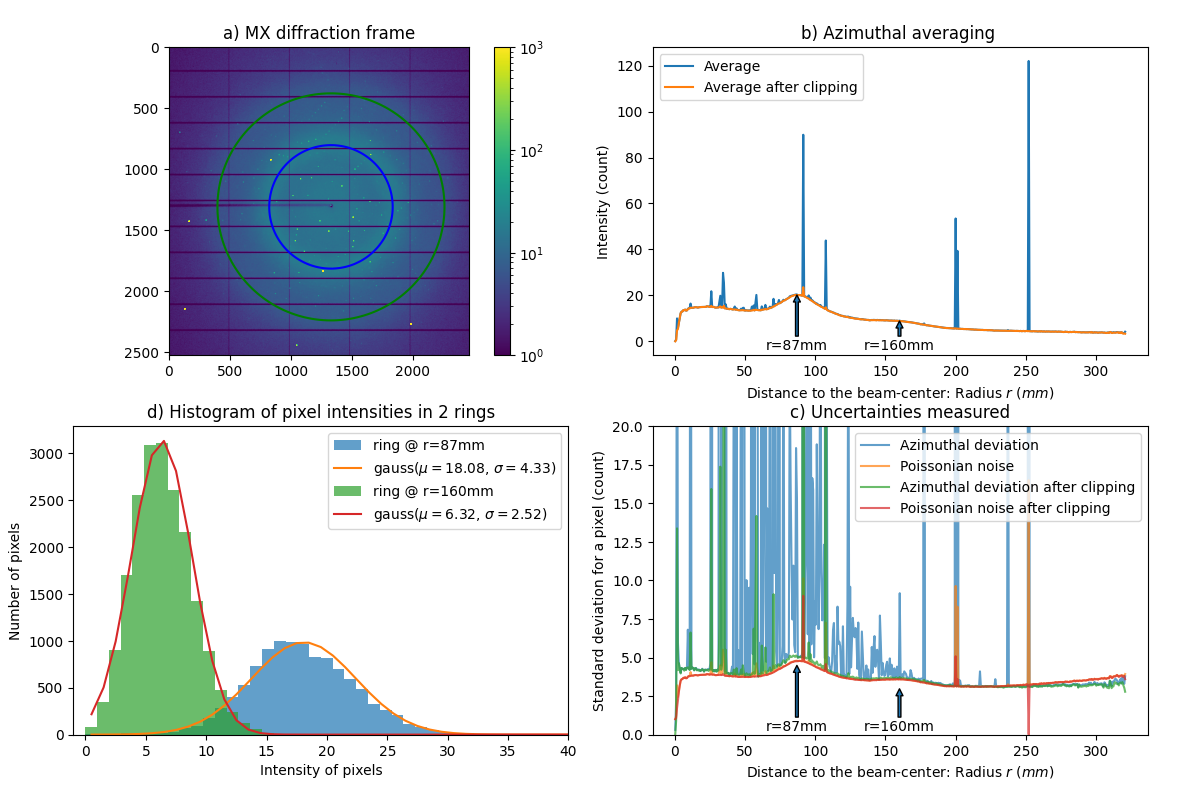
\includegraphics[width=14cm]{fig1}
\caption{Single crystal diffraction frame obtained from insulin with a Pilatus 6M (a) with the azimuthally averaged signal (b), 
before and after clipping data. Uncertainties are presented in (c) when calculated assuming a Poissonian error model (orange, red) or when measuring the deviation within all pixels in a ring (green, blue).
Subplot (d) presents the histogram of intensities for two rings at r=87mm and r=160mm from beam center with the distribution fitted as Gaussian curves: $g(x)\propto exp(-\frac{(x-\mu)^2}{2\sigma^2})$.}
\end{center}
\end{figure}

The core idea of the algorithm for background extraction is to model the distribution of background pixels. Unlike Bayesian statistics \cite{Sivia2006} where the cost function is usually tuned to weight less outlier, here, those outliers are simply flagged and discarded.
Positive outliers can reasonably be assigned to Bragg peaks and negative outliers to shadows or defective pixels. 
The distribution is recalculated  after discarding pixels for which intensity differ from the average value by more than $n$ times the standard deviation (Eq. \ref{clip}), where $n$ is called the Signal to Noise Ratio (SNR).
This clipping re-centers the distribution of remaining pixels since the mean is sensitive to outlier values:
\begin{equation}
\label{clip}
|I - <I>| > n \cdot \sigma(I)
\end{equation}
The orange plot in figure \ref{fig1}b presents the average after having discarded those outliers, and the orange and green curve of figure \ref{fig1}c are the uncertainties calculated after this clipping. 
After clipping, the average and uncertainties curves have lost most of their spikes, which means that most Bragg peaks and shadowed pixel have been discarded.

\subsection{Sigma-clipping}
The \textit{sigma-clipping} algorithm consists in applying this outlier rejection several times.
If the initial distribution is mono-modal, this algorithm enforces gradually the data to be sampled symmetrically around the maximum probability, which is likely to look like a normal distribution.
If the initial distribution is more complicated (typically multi-modal), the necessary larger standard-deviation will prevent most outlier pixels from being rejected, making it more conservative.
The sigma-clipping algorithm takes two parameters: the number of iterations and the rejection cut-off (SNR).
%I merged number of iterations and sigma clipping  as closely connected.
Despite the execution time is proportional to the number of iteration of sigma-clipping, iterations should continue until no more outliers are found, so that the background data can be treated assuming a normal distribution. 
Since the loop exits as soon as no more outliers were discarded at the clipping step, having an arbitrary large number of iteration is not really an issue for the execution time and the number of actual iteration is usually few (3 is commonly observed).       

\subsubsection{Limits of the Poissonian approach:}
%this will probably be discussed a lot by the reviewers, or completely ignored :P GS

The evaluation of uncertainties based on the variance within a radial shell (azimuthal model) has been developed after numerical artifacts were discovered while performing sigma-clipping with a Poissonian approach. 
Some azimuthal bins were showing no pixel contribution at all and thus appeared without any mean nor uncertainties, jeopardizing the complete background extraction algorithm. 
This artifact was directly linked to the usage of Poisson statistics and can be demonstrated with a simple distribution of 2 pixels, having values 1 and 199. 
The mean of this distribution is 100 and the standard deviation is also close to 100 while the uncertainty derived from a Poissonian law would  be close to 10 (i.e. $\sqrt{100}$). 
With the azimuthal error model, both pixels are a $1\sigma$ from the mean while with the Poissonian error-model, pixels are at $10 \sigma$.  
This explains why bins featuring strong Bragg-peaks on top low background got completely emptied from any contributing pixels when sigma-clipping was performed assuming Poissonian noise.

Unlike the Poisson error-model, the uncertainties obtained from the azimuthal-model are resilient to diffraction data coming from several types of samples but show much more variability from one bin to its neighbor (Fig. \ref{fig_std}). 
PyFAI introduces an \textit{hybrid} error-model which uses the azimuthal error-model for the sigma-clipping stage which trims the ensemble of pixels to become mono-modale.
The uncertainties are then calculated using a the Poisson error-model on the trimmed ensemble.

\subsubsection{Clipping threshold}
can be automatically calculated based on a variation on Chauvenet's criterion \cite{chauvenet} where one would accept to discard only a single pixel in a ring with a signal already following a normal law. 
Thus, the threshold value is adapted to the $size$ of the distribution, i.e. the number of pixels in each ring (Eq. \ref{chauvenet}), which can reach several thousands and shrinks with iterations.
Typically the numerical value for this cut-off varies from 2 to 4.   
\begin{equation}
\label{chauvenet}
SNR_{chauv.} =  \sqrt{2 log(\frac{size}{\sqrt{2 \pi}})}
\end{equation}

The worse case scenario for sigma-clipping corresponds to an initial distribution very far from a normal distribution, as the bimodal distribution seen in the previous paragraph.
Another challenging situation occurs close to the detector corners where the background signal is low and the size of the distribution is decreasing. 
For example this cut-off parameter increases from 2.7 to 3.5 when the size of the ensemble increases from 100 to 1000 elements.
% If the ensemble counts 100 (respectively 1000) pixels, the automatic clipping parameter evaluates to $SNR_{chauv.} = 2.7$ (respectively $SNR_{chauv.} = 3.5$).
So, for a Poissonian detector and a low count rate of one ($\lambda = \mu = \sigma^2 = 1$), any pixel with intensity greater than 4 is discarded with the ensemble of 100,  greater than 5 for the ensemble of 1000 pixels.
% could be interesting to show Threshold vs cycle for the example above (if relevant)
%it is relevant, but the paper is quite dense already

\section{Application to single crystal diffraction image compression}
Diffraction images from a single protein crystal exhibit usually an isotropic background on top of which Bragg peaks appear.
The sigma-clipping algorithm can be used to select the background level and more importantly the associated uncertainty.

This lossy compression algorithm consists in picking (and storing) pixels which intensity is above the average background value ($\mu$) plus $n$ standard deviation ($\sigma$). 
This cut-off value $n$ (also called $SNR_{pick}$) controls the amount of data to store and provides also a hint for the compression ratio achievable, assuming a normal distribution has been enforced at the sigma-clipping stage: 16\% of the pixel are to be recorded with $n=1$;  2.3\% for $n=2$ and only 0.13\% for $n=3$ as depicted in figure \ref{distribution}.
\begin{figure}
\label{distribution}
\begin{center}
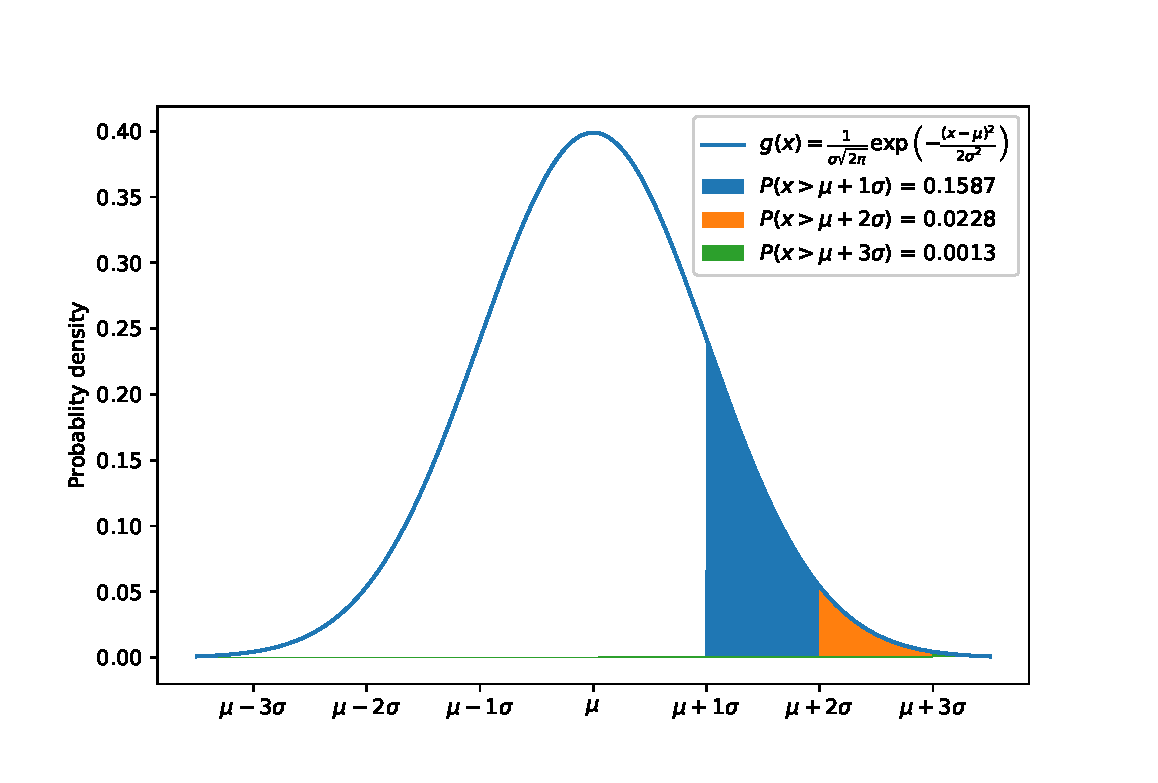
\includegraphics[width=9cm]{distribution}
\caption{Normal distribution and probability of having pixels with intensity above certain thresholds.}
\end{center}
\end{figure}

The storage space is much larger than just the pixel intensity since one needs to store as well its position in detector coordinates. 
Since diffraction analysis software are performing some kind of noise-level analysis, the background signal has to be regenerated with intensity and noise similar to the original data.
Thus, the average intensity per azimuthal bin together with the associated uncertainties needs to be stored.

\subsection{Sparsification}

The sigma-clipping algorithm was originally written for real-time sparsification of single crystal diffraction data and its integration into the LIMA2 detector control system \cite{lima} for the \textsc{Jungfrau} 4M detector used at ESRF ID29 is described in \cite{sri2021}.
The real-time constrain imposed to develop code running on GPU since those devices are several times
faster than equivalently priced processors.
All algorithms were developed in OpenCL \cite{opencl_khronos} and implemented in the \textit{pyFAI} software package (MIT-licence, available on github).
A command line tool called `sparsify-Bragg' is available for testing off-line since version 2023.01.

All the pixel coordinates and intensities are stored in a HDF5 container \cite{hdf5} following the NeXus  convention \cite{nexus}, together with a snippet of Python code explaining how to rebuild the dataset.
All sparse datasets (averaged and uncertainties curves, pixel coordinates, etc..) are compressed with the bitshuffle-LZ4 \cite{bitshuffle} lossless compression.

\subsection{Densification}
Since no crystallographic software package can deal with this sparse format (yet), the densification code was developed to regenerate initial frames and the `densify-Bragg` program was made available as part of the FabIO \cite{fabio} software package (MIT license). 
The source code is available on github and `densify-Bragg` is available since version 2022.12, available via usual channels like pip or conda install. 
The software constrains for this densification code are very different from the one for sparisfication since this code can be used by the final users.
For this reason `densify-Bragg' was optimized to run on multi-core CPU.
%option is probably not the right term here. 
Maybe an important consideration is whether, regardless from the file format, it is necessary to reconstruct the background or not. 
% Beside classical options like file-format and file-name, there is one important consideration whether the background noise has to be reconstructed or not. 
In fact, some crystallographic reduction program like CrysAlisPro \cite{crysalis} provide a better result with noise-less background while XDS \cite{xds}, which performs a deep noise analysis, needs to have the noisy background properly restored.
Shaded regions are never reconstructed properly and should be masked adequately in the reduction software.

Future development will focus on a HDF5-plugins able to provide access to densified images from their sparse representation. 
This will allow any analysis software able to read HDF5 files to treat sparse data as if they were dense, removing the burden of densifying the images from the users.

\subsection{Performances}
The performances for a lossy compression algorithm are to be evaluated along many directions: compression and decompression speeds, compression ratio and degradation of the recorded signal.
In the following example we present the sparsification of a Lysozyme (HEWL) dataset obtained using a traditional oscillation data-collection. 
Data were collected on an Eiger 4M detector \cite{lysozyme}, selected for its similarity in size and performances with the \textsc{Jungfrau} detector.
Those data are then densified again to regenerate the data and processed in XDS \cite{xds}.
Data quality indicators are finally compared between the original dataset and the one which went through the lossy compression presented here.

%This reference dataset is the one made publicly available by Dectris \cite{lysozyme} (TODO). 

\subsubsection{Compression ratio} 
After sparsification (picking cut-off: $2\sigma$, error-model: Poisonnian), the dataset still weights 103MB which represents a 15x compression ratio compared to the standard procedure.
For conformance with the state of the art, the reference dataset was re-compressed using the bitshuffle-LZ4 algorithm \cite{bitshuffle}, for which the 1800 frames weight 1500MB (instead of the 5000GB of the original files compressed in LZ4).

The maximum theoretical compression ratio for $2\sigma$ is 22x (figure \ref{distribution}, neglecting the storage of the background data and effects of the lossless compression).
To evaluate the effective maximal compression ratio, the dataset was median-filtered along the image stack to produce an image without peaks. 
A background dataset of 1800 such images sparsifies into a 11MB HDF5 file which represents a compression ratio of 136x ! 
Indeed, only 19 pixels were saved per frame and the compressed numerical values are mostly the same, which compresses great with bitshuffle-LZ4.

In production conditions, one would like to tune this threshold to the minimal value which guarantees a compression ratio large enough to allow the storage of all data.
For ESRF-ID29, where a \textsc{Jungfrau} 4M can operate close to 1 kHz, the pedestal+gain pre-processing convert 16-bits integers into 32-bits floating point values, doubling the bandwidth for data saving. 
The detector outputs the data via $8\times$ 10Gbit/s network links and the storage is performed via a single 25 Gbit/s link, making a minimum compression ratio of 6.4x which is equivalent to a cutoff at $1.4\sigma$ (cf. figure \ref{distribution}).


\subsubsection{Compression speed:}
%\begin{verbatim}
%kieffer@scisoft14:~/Dectris/EIGER_X_4M_lyso/demo$ sparsify-Bragg ../collect_01_00001_master.h5 -p ../geometry.poni  --bins 500 --unit="r_mm" --cycle=5 --cutoff-clip=0  --noise=1 --profile -m ../mask.npy --cutoff-pick=2.0 --error-model=poisson -o sparse.h5
%INFO:pyFAI.method_registry:Degrading method from Method(dim=1, split='pseudo', algo='histogram', impl='*', target=None) -> Method(dim=1, split='bbox', algo='histogram', impl='*', target=None)
%INFO:pyFAI.geometry:Unable to parse ../geometry.poni as JSON file, defaulting to PoniParser
%WARNING:pyFAI.ext.splitBBoxCSR:Pixel splitting desactivated !
%INFO:silx.opencl.processing:379.313MB are needed on device: TITAN V,  which has 12652.839MB
%INFO:silx.opencl.processing:Compiling file ['silx:opencl/doubleword.cl', 'pyfai:openCL/preprocess.cl', 'pyfai:openCL/memset.cl', 'pyfai:openCL/ocl_azim_CSR.cl', 'pyfai:openCL/peak_finder.cl', 'pyfai:openCL/peakfinder8.cl'] with options -D NBINS=500  -D NIMAGE=4485690 -D WORKGROUP_SIZE=1024
%INFO:silx.opencl.processing:■■■■■■■■■■■■■■■■■■■]  100%  Saving: sparse.h5                      
%OpenCL kernel profiling statistics in milliseconds for: OCL_PeakFinder
%                                       Kernel name (count):      min   median      max     mean      std
%                                 copy H->D indices (    1):    3.730    3.730    3.730    3.730    0.000
%                                  copy H->D indptr (    1):    0.001    0.001    0.001    0.001    0.000
%                                    copy H->D mask (    1):    1.096    1.096    1.096    1.096    0.000
%                                copy H->D radius1d (    1):    0.002    0.002    0.002    0.002    0.000
%                                copy H->D radius2d (    1):    3.489    3.489    3.489    3.489    0.000
%                               copy raw H->D image ( 1800):    3.615    5.064    5.718    4.893    0.412
%                                 cast u32_to_float ( 1800):    0.070    0.075    0.103    0.074    0.001
%                                         memset_ng ( 1800):    0.004    0.004    0.010    0.004    0.000
%                                       corrections ( 1800):    0.169    0.171    0.178    0.172    0.001
%                                   csr_sigma_clip4 ( 1800):    3.077    3.230    4.140    3.267    0.133
%                                    memset counter ( 1800):    0.004    0.004    0.015    0.004    0.001
%                                       peak_search ( 1800):    0.261    0.263    0.272    0.263    0.001
%                                 copy D->H counter ( 1800):    0.001    0.001    0.010    0.001    0.000
%                  copy D->D + cast uint32 intenity ( 1800):    0.007    0.010    0.025    0.010    0.002
%                           copy D->H peak_position ( 1800):    0.003    0.006    0.029    0.009    0.005
%                           copy D->H peak_intensty ( 1800):    0.003    0.006    0.029    0.009    0.005
%                          copy D->H background_avg ( 1800):    0.002    0.002    0.004    0.002    0.000
%                          copy D->H background_std ( 1800):    0.002    0.002    0.003    0.002    0.000
%________________________________________________________________________________
%                       Total OpenCL execution time        : 15687.401ms
%\end{verbatim}

The compression speed has been measured on the computer designed for online data-reduction of the \textsc{Jungfrau} detector \cite{sri2021}: 
an IBM AC922 using two Power9 processors and two (with possibility to upgrade to four) Nvidia Tesla V100 GPU. 
%add core counts for the single processor GS
The sequential execution of the code on the GPU takes about 4 ms to process one image and uses one single CPU-core and a quarter of a GPU. 
In online condition, multiple parallel processes are expected to achieve much higher frame-rate, since the nominal speed for the \textsc{Jungfrau} is 1kHz.

\subsubsection{Decompression speed:} 
The decompression of those data should typically be performed on a standard workstation (here running two Intel Xeon Gold 6134 CPU @ 3.20GHz): the reconstruction speed is found to take 30 s for the full dataset, while writing of the densified dataset (with bitshuffle-LZ4 compression) takes 45s. 
Densification is thus faster than writing on disk.
The reading time of the input sparse dataset is negligible (<2s).

\subsubsection{Quality of the restored dataset:} 
The densified dataset was processed via XDS and the summary indicator for the quality of the results are compared with the one coming from the reduction of the original dataset. 
Since those integrator are measured on integral peaks with $I/\sigma>3$ and the sparsification was performed
with a cut-off of 2, those result should be almost unaffected, which is confirmed in the table \ref{xds_summary}.

\begin{table}
\label{xds_summary}
\caption{Quality indicators after peak integration and averaging using XDS \cite{xds}. 
Lysozyme (HEWL) dataset provided by Dectris for advertising their Eiger-4M detector \cite{lysozyme}.}.
\begin{tabular}{|c|c c c|c c c|} 
\hline
Indicator & \multicolumn{3}{c|}{Initial dataset} & \multicolumn{3}{c|}{Lossy compressed dataset ($2\sigma$)} \\ 
          & 2.91\AA & 2.06\AA & all & 2.91\AA & 2.06\AA & all \\
\hline
Completeness                                        & 98.8& 90.8 & 93.8\% & 99.8& 90.6 & 93.5\% \\ 
$R_{obs}=\frac{\sum |I_{h,i}-I_{i}|}{\sum I_{h,i}}$ & 9.9 & 57.3& 12.5\% & 9.2 & 61.2&  11.4\%\\ 
$R_{expected}$                                      & 8.8 & 73.2& 15.0\% & 8.2 & 68.7 &  12.1\%\\
$R_{meas}$ \cite{Rmeas}  &10.3 &61.2& 13.2\% & 9.6 & 65.5 & 12.0\%\\
$CC_{1/2}$ \cite{cc1/2}  & 99.7 &94.0 & 99.7   & 99.6 & 95.4 & 99.7  \\
$<I/\sigma>$               & 25.80 & 5.39 & 10.52  & 26.33& 4.09 & 10.17 \\
\hline
\end{tabular}
\end{table}
%didn't we also refine data against the two datasets for comparison? GS
Those results are very different from the one described in \citeasnoun{veto_2024} where such lossy data compression technique is described as detrimental for the quality of the reduced data. 
The main difference between the two approaches is that here, no peak identification is performed, thus no minimum number of contiguous and intense pixels are to be found. 
So more pixels values get saved, trading disk space for quality of the recorded dataset.

\section{Application to serial crystallography}
A classical way of pre-processing serial-crystallography data is to shrink the amount of data by sieving-out empty or bad frames, only keeping the frames which deserve processing. 
This is the role of the "veto-algorithms".

The sigma clipping algorithm provides us with the background (average and deviation) and is used to pick pixels which are likely to be Bragg peaks. 
For this,  several additional checks are performed on the local neighbourhood which is a small square patch (typically 3x3 or 5x5 pixels):
\begin{itemize}
\item The considered pixel is the maximum of the local neighborhood.
\item Enough of pixels in the local neighborhood satisfying the SNR condition: typically 2 to 5 pixels out of 9 or 25 are intense enough.
\end{itemize}

For each peak, the pixel coordinate, the precise centroïd, the sum of data and its propagated deviation are recorded and reported. 
Those peak-position are saved into a HDF5 file (represented figure \ref{silx}) following the CXI format \cite{cxi} which can be can be read from CrystFEL \cite{CrystFEL}.
CrystFEL is the most popular software to process serial crystallography data, allowing to swap peak-picking algorithms \cite{zaefferer, Cheetah2014, robustpeakfinder} and indexing tools \cite{xds, mosflm, taketwo, xgandalf, pinkindexer}.
Since indexing is compute intensive, CrystFEL can distributes calculation over several cores or nodes.

\begin{figure}
\label{silx}
\includegraphics[width=12cm]{silx_view}
\caption{Peak-picking CXI-file produced by pyFAI and visualized with the \textit{silx viewer} \cite{silx}.
The left-hand side contains the HDF5 tree structure while the right-hand side presents the default plot with the number of peaks found per frame.}
\end{figure}

%not sure if the jump between previous and current sentence is too sudden GS
The serial crystallography beamline at the ESRF (ID29) uses a LImA2 monitor \cite{lima2} as visualization tool.
It is inspired from  NanoPeakCell \cite{nanopeakcell} for online visualization and feeds back information to check if peaks found correspond actually the crystal lattice expected for the sample.
We will first compare the peak-picking algorithm with some reference implementation on a single frame before evaluating the quality of the picked points on a serial-crystallography dataset where the indexation rate will be used as quality indicator.

\subsection{Comparison of picked peaks}
Figure \ref{peakfinder} presents the comparison between the original \textit{peakfinder8} described in \citeasnoun{Cheetah2014}, interfaced in Python via OnDA \cite{onda} and the version implemented into pyFAI on the same Pilatus 6M image, already used in figure \ref{fig1}. 

\begin{figure}
\label{peakfinder}
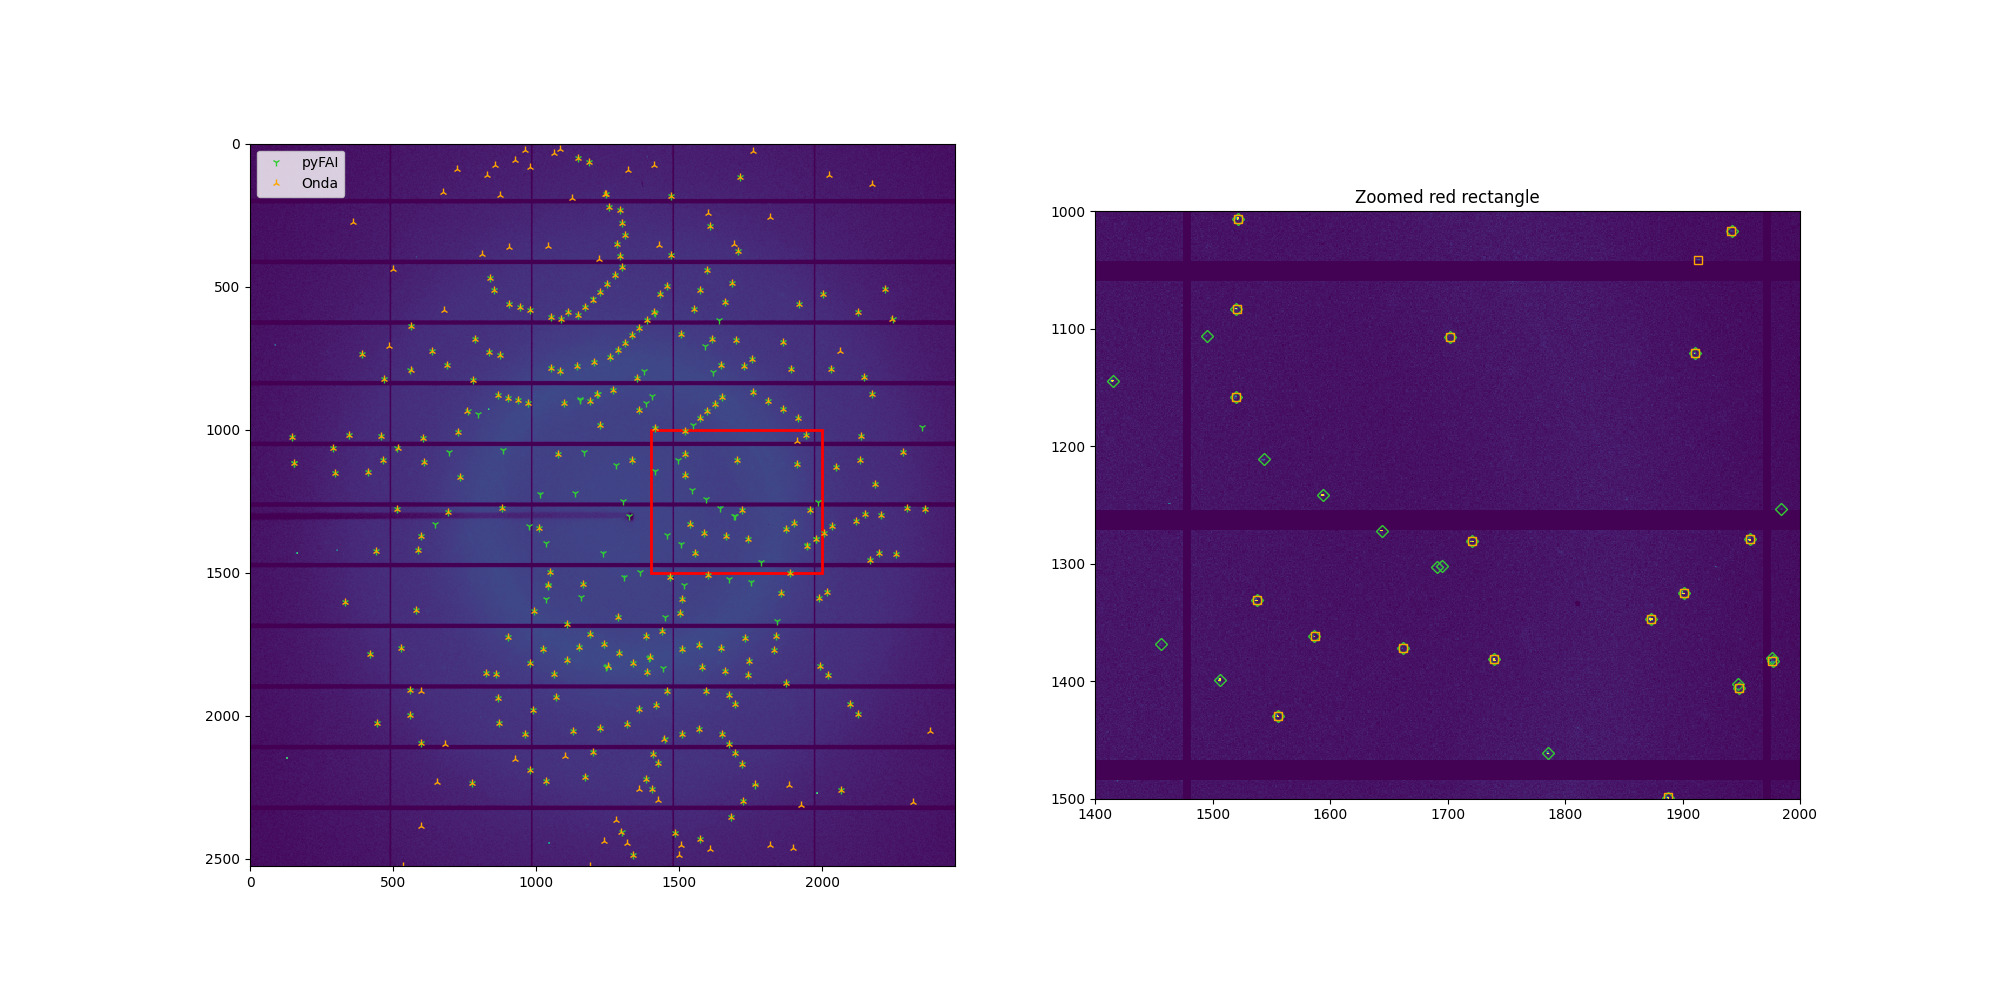
\includegraphics[width=12cm]{peakfinder}
\caption{Comparison of the reference \textit{peakfinder8} interfaced with Onda (in orange, execution time 300ms) and the version from pyFAI (in green, execution time 10ms) on top of a Pilatus 6M diffraction frame of an insulin crystal.}
\end{figure}

In figure \ref{peakfinder}, most peaks found by both implementation match and superimpose with Bragg-peaks.
There are more green peaks (found by pyFAI) closer to the beam center while more orange peaks (found by Onda) are located in the outer-shell.
This plot was made with a minimum SNR of 3 and a noise level of 1 since the Pilatus detector is Poissonian.
%no previous specification of which dataset we are using here!! GS
Peaks were registered if four pixels meet the SNR criterion in a 5x5 pixels patch around the peak.
Those parameters have been tuned to obtain a comparable number of peaks with both implementations: 290 with pyFAI and 293 with Onda.
The similarity of those figures allows a direct comparison of peaks found per resolution shell, histogram plotted in figure \ref{peak_per_ring}.

\begin{figure}
\label{peak_per_ring}
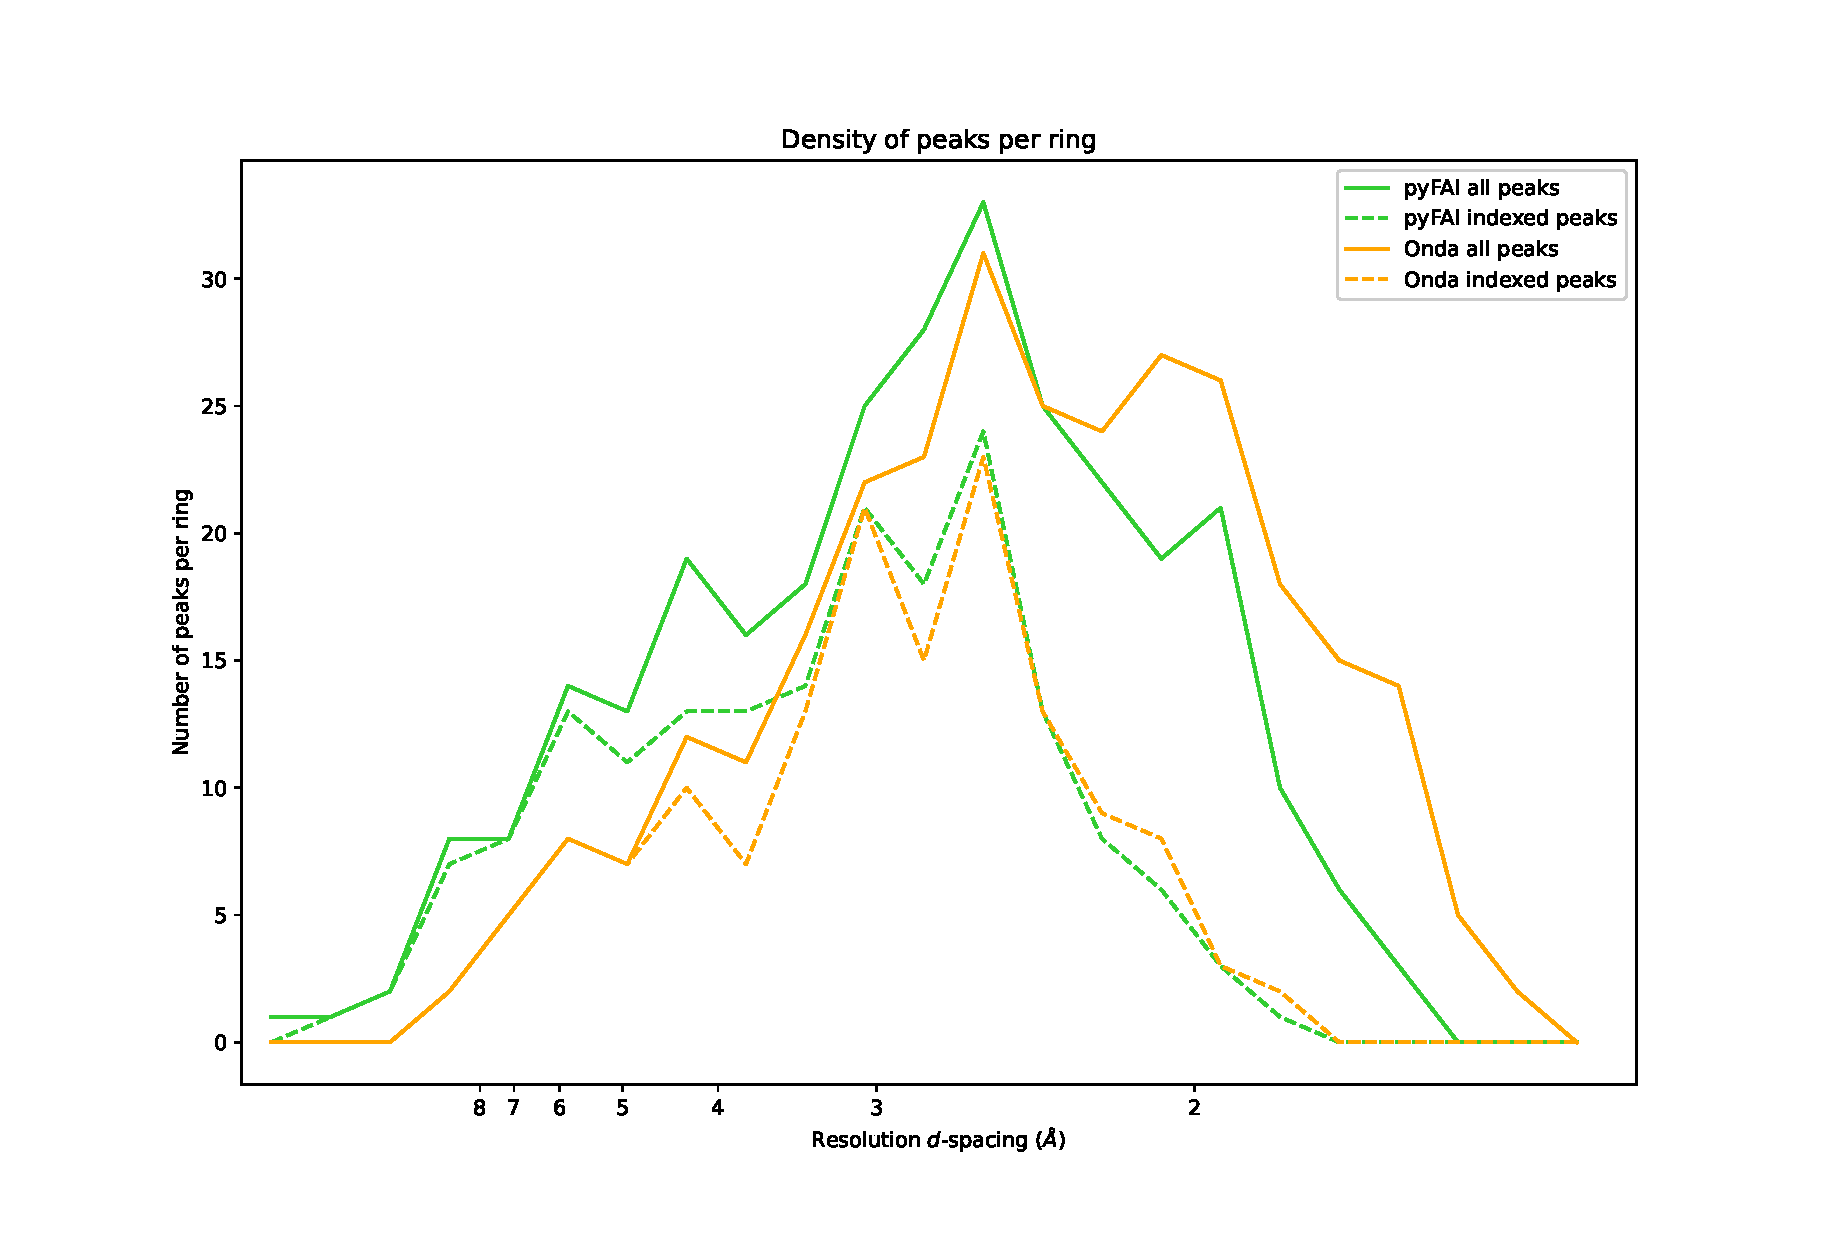
\includegraphics[width=12cm]{peak_per_ring}
\caption{Number of peaks found in the different resolution shell for the \textit{peakfinder} implemented in pyFAI and in Onda. 
The width of each radial-shell is two inverse nanometer in $q-$space. 
The dashed lines represents the number of those peaks which have successfully been indexed, i.e. located at less than two pixels away from an expected reflection (calculated by Xgandalf). }
\end{figure}

The figure \ref{peak_per_ring} presents the histogram of modulus of the scattering vector of the peaks found with different methods, i.e. the number of peaks having a given q-value.
For readability, those histograms (bin width: $2 nm^{-1}$) have been represented as plots with the horizontal axis labeled in d-spacing ($q=2\pi/d$).  
The analysis of those histograms confirms that the implementation in pyFAI is getting more points closer to the beam-center while the reference implementation is picking more point at larger q-values.
This is likely due to the curvature of the Debye-Scherrer ring: the original version of peakfinder8 evaluates the variance in a neighborhood defined by some radius around the point of interest and the variance is higher close to the beam-center due to the important curvature of those rings.
On the opposite, pyFAI knows about this curvature and measures the variance along the ring.
Points picked by Onda at larger q-values do not look like Bragg-peaks but this could be a side-effect of the parameter tuning to get the same number of peaks for both algorithms.

The same figure presents with dashed lines the number of peaks which are coincident (within 2 pixels) with expected reflections (after indexing using Xgandalf).
It demonstrates that the additional peaks found by pyFAI in the inner-shell ($d>3\AA$) are consistent with Bragg-peaks, thus valuable for indexing, while the additional peaks found by Onda in the outer shell ($d<2\AA$) are not Bragg-peaks, and thus are detrimental.

A word on performances: the Python binding in Onda to the peakfinder8 algorithm from Cheetah runs in 180ms on a high-end server CPU (AMD Epyc 7262) and 300ms on a workstation (Intel Xeon E5-1650 v4). 
The version available in pyFAI was designed in OpenCL \cite{opencl_khronos, opencl, pyopencl} and runs best on GPUs: 30ms on a AMD Vega 56 and in 10 ms on a Nvidia RTX A5000. 
Interestingly, an entry level GPU (Nvidia GT1030), which is seven times cheaper than the Epyc processor, shows the same performances (but this CPU has eight cores). %curiosity, not sure if relevant for the discussion GS

\subsection{Quality of the peakfinder on serial crystallography data}
\label{quality-pf}
The quality of peaks extracted with this algorithm is finally evaluated on a serial-crystallography dataset: tiny crystals of egg white lysozyme (HEWL) were deposited on a SiN membrane and this membrane was scanned in front of the beam at the ID30A3 beamline at the ESRF with an Eiger 4M detector.%check BL, could be id13 if it's the data from Coquelle 20014
A fraction of 1000 frames of the dataset %\cite{ssx-Lyso} 
was used as a probe and was indexed with the $indexamajig$ tool from CrystFEL. 
Since all frames show Bragg-peaks (figure \ref{silx}) the number of indexed frames can be seen as a quality indicator of the peak-picking algorithm used, when all other parameter remain unchanged.
The indexation was performed with the \textsc{xgandalf} algorithm \cite{xgandalf} with default settings from CrystFEL 0.10.1 and was provided with the cell parameter: tetragonal $a=b=78.77\text{\AA}; c=39.04\text{\AA}; \alpha=\beta=\gamma = 90^o$.
The table \ref{crystfel} compares the number of frames properly indexed with the different picking algorithms available in CrystFEL and with the algorithm presented here. 

\begin{table}
\label{crystfel}
\caption{Indexation rate obtained with \textsc{xgandalf} \cite{xgandalf} from peak positions extracted with different picking algorithms available from CrystFEL \cite{CrystFEL} on a subset of 1000 frames of microcrystals of Lysozyme (HEWL) collected with an Eiger 4M at ESRF-ID30A3.}%there is no Eiger on 30B,data could be from 30a3 or id13. Check with Nico GS
\begin{center}
\begin{tabular}{|c|c|c|c|c|} 
\hline
Peak-picking  & \multicolumn{2}{c|}{\textsc{xgandalf} (default)} & \multicolumn{2}{c|}{\textsc{xgandalf} (fast)}\\
method & Index. rate & run-time & Index. rate & run-time \\ 
\hline
Zaef \cite{zaefferer} & 10.0\% & 2178 s & 10.0\%& 430 s\\
PeakFinder8 \cite{Cheetah2014} & 49.5\%& 10397 s &48.5\% & 1757 s\\
PeakFinder9 \cite{FDIP} & 44.2\%& 8328 s&43.5\%&1436 s\\
RobustPF \cite{robustpeakfinder} & 22.4\%& 6314 s& 21.2\%& 1628 s \\
pyFAI (this contribution) & 49.7\%& 9325 s& 49.2\% &1595 s\\
\hline
\end{tabular}
\end{center}
\end{table}

Since the Eiger detector is a counting detector, the global threshold for algorithms \textit{zaef} and \textit{peakfinder8} had to be lowered (to 50, which is the maximum of the background signal on any frame) and the the default SNR value was used for \textit{zaef}, \textit{peakfinder8}. 
The same SNR value of five was used for \textit{pyFAI}.
%also because default parameters are tuned for XFEL bragg peak values!
Default parameters were used for \textit{PeakFinder9} and \textit{RobustPeakFinder} algorithms.
The reported run-time correspond to the execution time on a single core of an Intel Xeon Gold 6134.


The indexing rate obtained with the algorithm from pyFAI is in par with the reference implementations like \textit{peakfinder8} or \textit{peakfinder9} available from CrystFEL. 
Since time is mostly spent in indexing, sets of peaks which are simpler to index present lower run-time as fewer retry were needed.
Retries can be deactivated but they increase significantly the success of indexing. 
Table \ref{crystfel} presents also the indexing performances when using the option \textit{--xgandalf-fast-execution} from \textit{indexamajig}, which is five to six times faster and exhibits a limited degradation of the indexing rate.
The peak extraction in pyFAI is about as fast as the sparsification, so it can be used online to perform the pre-analysis and provide peaks to NanoPeakCell. 
Nevertheless the executable `peakfinder` available from pyFAI (offline tool) has a total execution time which is much larger: about 30 s for 1000 frames, most of which is spent in reading and writing the different HDF5 files.

\subsection{Peak count as $veto$ algorithm}
Since the background extraction and peak finding are performed in real-time on the serial-crystallography beamline ID29 at ESRF, the information about the number of Bragg-spots can be used to assess the quality of each individual image and the acquisition system can decide to discard the frame depending on the number of peaks and a live-adjustable threshold. 

Since the beginning of operation of ESRF-ID29, in 2022, the beamline operated with the $veto$ algorithm deactivated, the number of peaks found was just recorded for future exploration. 
The figure \ref{veto-fig} presents the indexation rate of "hit" (in blue) and "non-hit" frames (in orange) when changing the threshold for the minimum peaks-count per frame. 
The expected compression rate is displayed in green.
The dataset consists of 80000 lysozyme micro-crystals between two mylar films, raster scanned with a x-ray beam of 11.56 keV at ESRF-ID29.
The offline analysis has been performed with CrystFEL (v0.11.0) using `peakfinder8` and `xgandalf` as indexer. 

\begin{figure}
\label{veto-fig}
\begin{center}
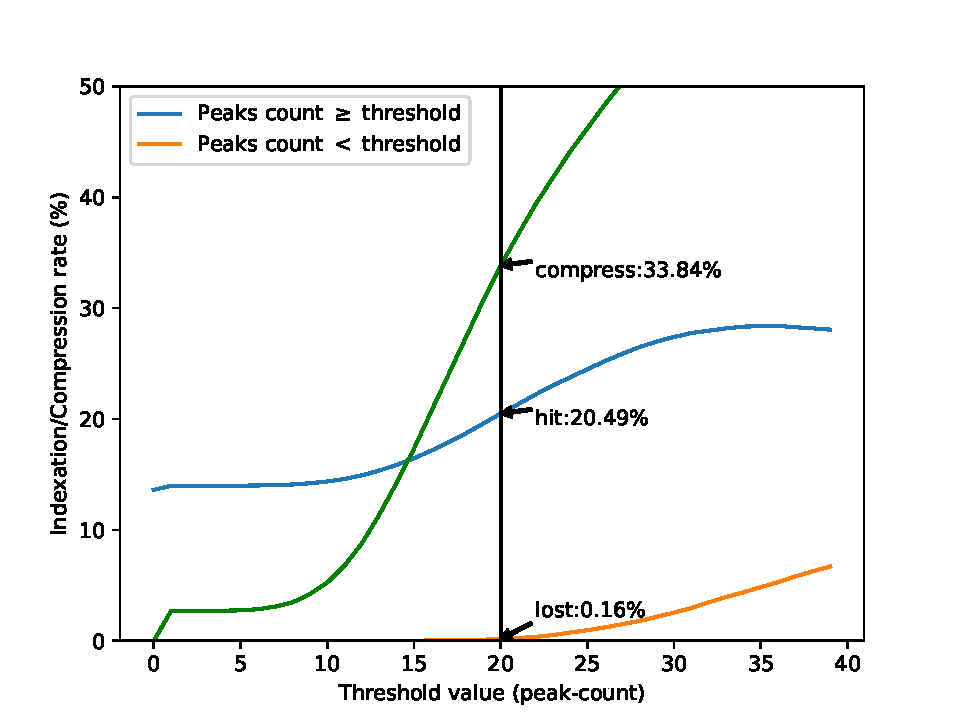
\includegraphics[width=9cm]{fig7/veto-fig}
\caption{Indexation rate of frames which would be considered as "hit" or "non-hit" as function of the peak-count threshold. 
The green curve presents the disk space which could have been saved.
The sample dataset consists of 80000 frames of lysozyme micro-crystals indexed off-line with Xgandalf in CrystFEL.}
\end{center}
\end{figure}

%summarized in the table \ref{veto-table}:

% \begin{table}
% \label{veto-table}
% \caption{Indexation rate for frames \cite{lysozyme}.}.
% \begin{tabular}{|c|c|c|c|} 
% \hline
%  & hit & no-hot & total \\ 
% Number of frames & - & - & 80000 \\
% Indexed & - & - & - \\
% Indexation rate & - & - & - \\
% \hline
% \end{tabular}
% \end{table}

Since the \textsc{Jungfrau} is an integrating detector, the detector has relatively more background noise than a photon counting detector: here, data were saved with 8 ADU/photon, making the compression rate of hit and non-hit frames similar.
In this example, discarding frames with less than 20 peaks of would have allowed to save one third of the network bandwidth and disk space, loosing only 0.16\% of frames index-able. 
The indexation rate of actually recorded frames also increased to 20\%.
The $veto$ algorithm having proved its robustness, it is now activated for (most) experiments on combination with a graphical helper tools to asses the optimal threshold during the experiment.


\subsection{Limitations}
There is a strong sensitivity of the indexation rate with data from the \textsc{Jungfrau} detector, related to the description of the detector in CrystFEL.
The \textsc{Jungfrau} 4M detector is built from 8 modules manually assembled and exhibits some residual  misalignment, on the order of a couple of pixels.
This misalignment is much larger than what has been measured on Eiger detectors from Dectris, where misalignment is less than one pixel in size (75 µm).
On Eiger detector data, where the detector is defined as a single rigid module, the indexation rate is fairly independent of the peak-picking algorithm as described in \ref{quality-pf}.
% Since the geometry of the detector used for the azimuthal integration is based on pyFAI, where every pixel is independent, it differs from the geometry used by the indexing software in CrystFEL where pixels are assembled in rigid modules.
% on the peak-position obtained either from pyFAI or from the integrated peakfinder8 code with 
% could explain the lower indexation rate of peaks position obtained with \textsc{Jungfrau} data in comparison with the Eiger data described in \ref{quality-pf}.
%), which could be linked to the detector geometric distortion and/or the pink beam. 
Work is ongoing to convert the geometry description from pyFAI, where every pixel is independent, to the geometry used in CrystFEL, and vice-versa.
Until then, frames are indexed on peak position freshly re-extracted by CrystFEL using its own peak-finding algorithms. 

\section{Conclusion}

Background analysis of single crystal diffraction images can be implemented efficiently using iterative azimuthal integration and allows the separation of the signal originating from Bragg-peaks from amorphous background.

A first application presented is lossy compression of diffraction frames where the average background is saved on the one side and the position and the intensity of pixels belonging to peaks on the the other.
The quality of the compression has been demonstrated on rotational macro-molecular crystallography where the degradation of the signal has been monitored after a cycle of compression-decompression and the analysis of those dataset with standard reduction tools (XDS).

The second application is a peak-finder for synchrotron serial crystallography which locates peak positions in real time and can be used to discard frames. 
The quality of the picking has been evaluated by comparing the indexation rate with reference peak-finder algorithms.
The number of peaks found is used as veto algorithm to discard frames without diffraction signal and save storage space.

     %-------------------------------------------------------------------------
     % The back matter of the paper - acknowledgements and references
     %-------------------------------------------------------------------------

     % Acknowledgements come after the appendices

\ack{Acknowledgements}
The authors would like to thank Andy G\"otz for the management of this project and Vincent Favre-Nicolin for his support.
Thanks also to Gavin Vaughan, scientist at Materials beamline at the ESRF,  for the constructive discussion about sigma-clipping versus median filtering.
We would like to thank also Jonathan P. Wright and Carlotta Giacobbe for offering us the ability to test those algorithms on small molecule data and validate the concept of sparsification on the ID11 beamline at the ESRF.
Pierre Paleo and Jerome Lesaint are also acknowledged for the fruitful discussions on numerical methods developed in this document.

\bibliographystyle{iucr}
\bibliography{biblio}

\end{document}                    % DO NOT DELETE THIS LINE
%%%%%%%%%%%%%%%%%%%%%%%%%%%%%%%%%%%%%%%%%%%%%%%%%%%%%%%%%%%%%%%%%%%%%%%%%%%%%%
